\section{Anforderungsanalyse}
\vspace{0,5cm}

Die gefundenen Anforderungen basieren auf den Inhalten des Lastenhefts, sowie der ersten Besprechung mit den Auftraggebern.


\subsection{Benutzerfunktionen}

\begin{itemize}
    \item \textbf{/F0010/}\textit{Formulare auswählen:} \par
    Ein Benutzer kann Formulare in den Menüs suchen und sich ein Formular anzeigen lassen.
    \item \textbf{/F0020/}\textit{Formulare ausdrucken:} \par
    Ein Benutzer kann ein gefundenes Formular über eine Schaltfläche in der Anwendung ausdrucken.
\end{itemize}
\vspace{1,5cm}
\textbf{Optional:}
    \begin{itemize}
        \item \textbf{/F0030/}\textit{Schnellsuche:} \par
        Der Benutzer kann durch Eingeben eines Suchbegriffs in eine Suchleiste den in der Datenbank hinterlegten Namen eines Formulars direkt suchen. Ist der Name hinterlegt, wird das entsprechende Formular zur Auswahl angezeigt.
        \item \textbf{/F0040/}\textit{eGK einlesen und Formulare vorausfüllen:} \par
        Wurde vom Benutzer ein Formular ausgewählt, kann er seine eGK an einem am IPad angeschlossenen Kartenlesegerät einlesen lassen. Das System füllt das ausgewählte Formular mit den ausgelesenen Daten des Benutzers.
        \item \textbf{/F0050/}\textit{persönliche Beratung durch Videoanruf:} \par
        Der Kunde kann an beliebiger Stelle des Prozesses durch einen Tastendruck einen Videoanruf mit einem Mitarbeiter der Filiale starten.
    \end{itemize}
    
\newpage

\subsection{Administratorfunktionen}

    \begin{itemize}
        \item \textbf{/F0110/}\textit{Einfügen von Formularen:} \par
        Ein Administrator kann Formulare im Format PDF in das Backend hochladen und speichern.
        
        \item \textbf{/F0120/}\textit{Bearbeiten von Formularen:} \par
        Ein Administrator kann die Metadaten eines hochgeladenen und gespeicherten Formulars, wie Titel oder Position in der Menüstruktur, direkt im Backend bearbeiten.
        
        \item \textbf{/F0130/}\textit{Löschen von Formularen:} \par
        Ein Administrator kann ein im Backend gespeichertes Formular aus dem Backend löschen.
        
        \item \textbf{/F0140/}\textit{Setzen der Farben und Logos:} \par 
        Ein Administrator kann die Farben des Frontends anpassen. Außerdem kann er Logos im jpg-Format hochladen und im Frontend anzeigen lassen.
        
        \item \textbf{/F0150/}\textit{Export und Import:} \par
        Die Einstellungen können als JSON Datei exportiert und importiert werden. Die Formulare werden zusammen mit der JSON-Datei in einer Menüstruktur exportiert.
    \end{itemize}{}
\vspace{1,5cm}
\textbf{Optional:}
    \begin{itemize}
        \item \textbf{/F0160/}\textit{Updates:} \par 
        Ein Administrator kann über eine zeitlich begrenzte Internetverbindung das System updaten.
        
        \item \textbf{/F0170/} \textit{Onlinekonfigurationsabgleich:} \par
        Ein Administrator kann den Abgleich der Einstellungen mit einem zentralen Server der Filiale starten.
    \end{itemize}
    
    \newpage
    
\subsection{Systemübersicht}

In Abbildung \ref{fig:UseCase} werden die Nutzungs- und Administrationsanforderungen des Systems sowie die Systemgrenzen als Use-Case-Diagramm dargestellt um einen übersichtlichen Gesamteindruck zu gewinnen.
\vspace{1cm}

\begin{figure}[htp]
    \centering
    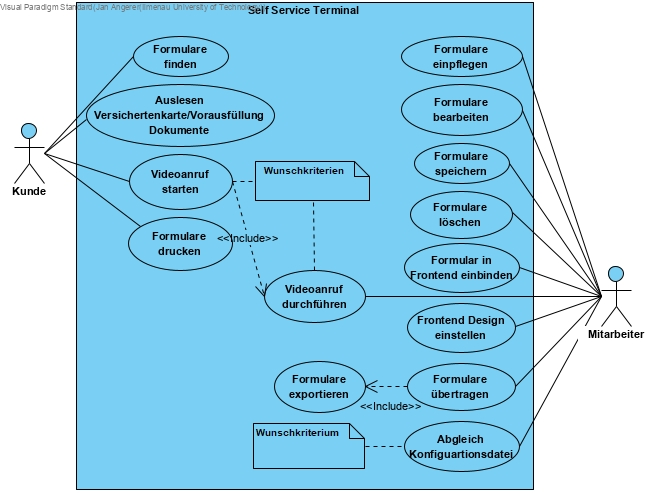
\includegraphics[width=15cm , height=13cm]{Kapitel/Bilder/USeCasev2.jpg}
    \caption{Systemübersicht}
    \label{fig:UseCase}
\end{figure}
\newpage

\subsection{Nicht Funktionale Anforderungen}

\vspace{1cm}

\begin{itemize}
    \item \textbf{/N010/} \textit{Intuitive Bedienbarkeit:} \par
    Die Benutzeroberfläche muss übersichtlich gestaltet werden. Dafür empfehlen sich bildschirmfüllende Schaltflächen mit kontrastreichen Farben. Es sollen nach Möglichkeit nicht mehr als fünf Schaltflächen pro Seite angezeigt werden. 
    
    \item \textbf{/N020/} \textit{Nur eindeutige Eingaben möglich:} \par
    Ein Nutzer soll nur Eingaben tätigen können, die eindeutig sind und genau das ausführen, was sie suggerieren.
    
    \item \textbf{/N030/} \textit{Hohe Performanz:} \par
    Die Reaktionszeit der Benutzeroberfläche beim Klick auf eine Schaltfläche soll dauerhaft unter einer Sekunde liegen.
    
    \item \textbf{/N040/} \textit{Zuverlässigkeit:} \par
    Es soll ein Dauerbetrieb möglich sein. Bei einem Ausfall von Clients soll das System sich automatisch neu starten und wieder lauffähig sein.
    
    \item \textbf{/N050/} \textit{Wartungsarmer Betrieb:} \par
    Einmal eingerichtet soll das System möglichst keine Administratoreingriffe benötigen, bis auf das aktuell Halten der Formulare und Einstellungen. Updates sollen nur in einem Zeitraum $> 3$ Monate nötig sein.
\end{itemize}{}
\newpage
\subsection{Randbedingungen}

\vspace{1cm}
\begin{itemize}
    \item \textbf{/R010/}\textit{Internetzugang:} \par
    Das System darf zum Betrieb keine Internetverbindung benötigen. Dies ist nur während eines Updateprozesses zeitlich begrenzt möglich.
    
    \item \textbf{/R020/}\textit{Betriebssystem:} \par
    Als Betriebssystem ist eine Debian basierte Linux-Distribution vorgegeben.
   
    \item \textbf{/R030/}\textit{Hardware:} \par
    Als Server wird ein \textit{Raspberry Pi} vorgegeben. Als Client fungiert ein \textbf{Apple IPad} mit einer Bildschirmdiagonale von 9 Zoll. Der Ausdruck der Dokumente erfolgt durch einen Netzwerkdrucker oder einen über USB am Server angeschlossenen Drucker.
  
    \item \textbf{/R040/}\textit{Lokales Netzwerk:} \par
    Das System \textit{Raspberry Pi, IPad, Drucker} befinden sich nicht im WLAN der Filiale. Der Pi erzeugt zur Kommunikation ein eigenes Drahtlosnetzwerk.
  
    \item \textbf{/R050/}\textit{Frontend:} \par
    Durch die Nutzung eines \textit{IPads} als Client, muss die Darstellung des Frontends auf dem Safari Browser möglich sein.
  
    \item \textbf{/R060/}\textit{Design:} \par
    Das System soll auch für Menschen Nutzbar sein, welche sich nicht mit Technologie auskennen. Das Nutzerinterface ist daher simpel und deutlich lesbar zu gestalten.
\end{itemize}